\section{Experiments}
\label{sec:expe}

In this part, we compare \Moca to the other existing tools for memory analysis. In a first time, we present their main differences in terms of portability
and capabilities. Then, we present two sequences of quantitative experiments, one that outlines the importance of the default parameters chosen for our tool
and the other that compares the precision and performance of all the tools.

%\newpage

\subsection{Methodology}
\label{sec:exp-methodo}

%This section briefly discusses our experimental setup for the evaluation of
%\Moca.

Our main experiments were run on  machines from Grid5000 \Edel
cluster.
    As some state of the art tools can only run on AMD machines, we also run
    some of the experiment presented in section~\ref{sec:expe-ovh} on
    \Stremi machine from grid5000 grenoble.
    These machines hardware specification is summarized in
    \tbl{tab:hw}\footnote{Grid5000 provides an online hardware description:\\
        \url{https://www.grid5000.fr/mediawiki/index.php/Grenoble:Hardware\#Edel}
        \\\url{https://www.grid5000.fr/mediawiki/index.php/Reims:Hardware\#Stremi}}.
%     \\\url{http://digitalis.inria.fr/index.php/Idfreeze}}.

\begin{table}[htb]
    \centering
    \begin{tabular}{lp{1.1cm}rrp{1.35cm}p{1.1cm}}
        \toprule
        \multirow{3}{.8cm}{CPU}
        &  & \multicolumn{2}{c}{Vendor} & \multicolumn{2}{c}{Model} \\
        \cmidrule(lr){3-6}
        & \Edel  & \multicolumn{2}{c}{Intel} & \multicolumn{2}{c}{Xeon E5520} \\
        % & \Idfreeze & \multicolumn{2}{c}{AMD} & \multicolumn{2}{c}{Opteron 6174} \\
        & \Stremi & \multicolumn{2}{c}{AMD} & \multicolumn{2}{c}{Opteron 6164 HE} \\
        \midrule
        \multirow{3}{.8cm}{System totals}
        & & Nodes & Threads & Freq & Memory \\
        \cmidrule(lr){3-6}
        & \Edel   & $2$ & $8$ & \SI{2.27}{Ghz} & \SI{24}{Gib} \\
        %& \Idfreeze & $8$ & $48$ & \SI{2.20}{Ghz} & \SI{256}{Gib}\\
        & \Stremi & $2$ & $24$ & \SI{1.7}{Ghz} & \SI{48}{Gib}\\
        \midrule
        \multirow{3}{.8cm}{Per node}
        & & Cores & Threads & L3 Cache & Memory \\
        \cmidrule(lr){3-6}
        & \Edel   & $4$ & $4$ & \SI{8}{Mib} & \SI{12}{Gib} \\
        %& \Idfreeze & $6$ & $6$  & \SI{12}{Mib} & \SI{32}{Gib} \\
        & \Stremi & $6$ & $6$  & \SI{12}{Mib} & \SI{24}{Gib} \\
        \bottomrule
    \end{tabular}
    \caption{Hardware configuration of our evaluation system.}
    \label{tab:hw}
\end{table}

For every experiment, we deployed the same \emph{Debian} \emph{Jessie}
environment running a \texttt{Linux 3.16.0-4} with hyper threading was
disabled. We disabled address space randomization to produce memory trace as
comparable as possible.  As our two evaluation machines are not equivalent in
terms of hardware, we limited the number of threads used by openMP to $8$
which is the number of threads available on \Edel machines.

\begin{table}[htb]
    \centering
    \begin{tabular}{p{1.3cm}lcc}
        \toprule
        & & Mechanisms* & Architecture \\
        \cmidrule(lr){3-4}
        \multirow{4}{.8cm}{Portability}
        & \TABARNAC & Inst & Intel, AMD \\
        \addlinespace
        & \Mitos & PEBS + Inst & Intel \\
        \addlinespace
        & \MemProf & IBS & AMD \\
        \addlinespace
        & \Moca & PfI (+ Inst) & \textbf{Any}\\
        \midrule
        & & Granularity & superset \\
        \cmidrule(lr){3-4}
        \multirow{4}{.8cm}{Trace precision}
        & \TABARNAC & Page & \textbf{Page} \\
        & \Mitos & \textbf{Address} & None \\
        & \MemProf & \textbf{Address} & None \\
        & \Moca & \textbf{Address} & \textbf{Page} \\
        \midrule
        & & \multicolumn{2}{C{5cm}}{Time, Thread sharing, CPU**} \\
        \cmidrule(lr){3-4}
        \multirow{4}{.8cm}{Additional information}
        & \TABARNAC & \multicolumn{2}{C{5cm}}{Thread sharing} \\
        \addlinespace
        & \Mitos & \multicolumn{2}{C{5cm}}{Time + CPU} \\
        \addlinespace
        & \MemProf & \multicolumn{2}{C{5cm}}{\textbf{All}}  \\
        \addlinespace
        & \Moca & \multicolumn{2}{C{5cm}}{\textbf{All}} \\
        \bottomrule
    \end{tabular}
    \caption{Comparison of different memory traces tools.
        %\TABARNAC~\cite{Beniamine15TABARNACRR},
        %\Mitos~\cite{Gimenez14Dissecting},
        %\MemProf~\cite{Lachaize12MemProf} and \Moca.
        \\
        \emph{*~Inst: Binary instrumentation, PfI: Pagefault Interception}\\
        \emph{**~CPU on which the access occured}}
        \label{tab:tools-comp}
\end{table}

We evaluate \Moca by comparing it to the following state of the art tools. The first one,
\Mitos, is the tracing tool from MemAxes~\cite{Gimenez14Dissecting} and relies on Intel
PEBS technology.
The second one, \TABARNAC~\cite{Beniamine15TABARNACRR}, is one of our previous contribution.
It is based on a Pin instrumentation, which traps all the memory accesses but 
only counts the number of time each thread accesses to each page.
Although this is less precise than the information collected by \Moca, it does not require
the management of large and complex data structures.
The third one, \MemProf~\cite{Lachaize12MemProf}, is designed to analyze NUMA
performance issues and relies on AMD IBS.
\tbl{tab:tools-comp} summarizes the main differences
between \Moca and these other memory profiling tools.

In the following sections, all the tools are
evaluated on each of the 10 \NPB~\cite{Jin1999}.
Each point in each plot is the average of at least $30$ executions. Along with each point,
the error bars represent the standard error.
Except for the experiment about the influence of \Moca's parameters, on each
experiment, \Moca has been run with it's default parameters: a wakeup interval of
\SI{0.5}{s} for the logging process and \SI{50}{ms} for the monitoring thread.


We consider experimental reproducibility as an important matter, therefore we
distribute\footnote{The three distribution are available on github:\\
    \url{https://github.com/dbeniamine/hpdc_expe}}
all the files needed to reproduce our experiments at three different levels:

\begin{enumerate}
    \item \textbf{Statistic analysis:} To reproduce our statistic analysis we provide
        the filtered results (csv files) from the experiments along with the
        \texttt{R-markdown} scripts that generated the plots presented in this
        article.
    \item \textbf{Raw traces analysis:} At this level, we provide the full raw traces
        generated by our experiments along with the scripts used to extract the
        filtered traces (csv files from the previous level) and the scripts used
	at the previous level to perform the analysis.
    \item \textbf{Complete experiment:} At the most comprehensive level, we provide a git
        repository that includes our deployment environment, dependencies to all the
        tools and files required and instructions that explain how
        to reproduce the experiment with or without access to grid5000.
\end{enumerate}


%\subsection{Experiments}
\subsection{Moca default parameters}
\label{sec:expe-param}

Before comparing \Moca to existing tools, we need to evaluate the impact of
the wakeup intervals (logging daemon and monitor thread) on the trace
precision and on the overhead. To do so, we run the \IS benchmark instrumented by \Moca with
a wakeup interval ranging from \SI{0.1}{s} to  \SI{0.9}{s} for the logging daemon and from \SI{20}{ms} to
\SI{100}{ms} for the monitoring thread. For each run, we measure \IS execution time and the number of
accesses captured. We have chosen \IS for this evaluation as it is one of the memory intensive \NPB,
quick experiments with other ones confirmed these results. This experiment was
run on a machine from the \Edel cluster.

\begin{figure}[htb]
    \centering
    \begin{subfigure}{\linewidth}
        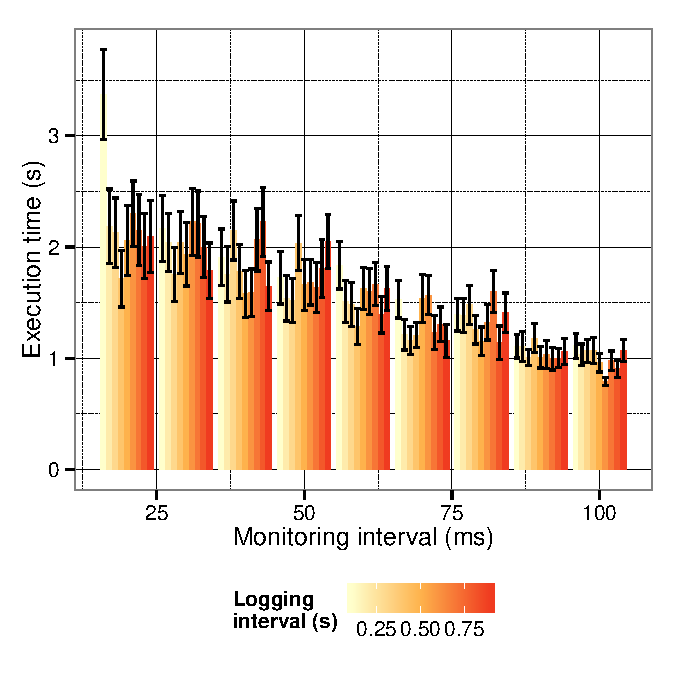
\includegraphics[width=\linewidth]{moca_param.pdf}
        \caption{Execution time.}
        \label{fig:param_time}
    \end{subfigure}
    \begin{subfigure}{\linewidth}
        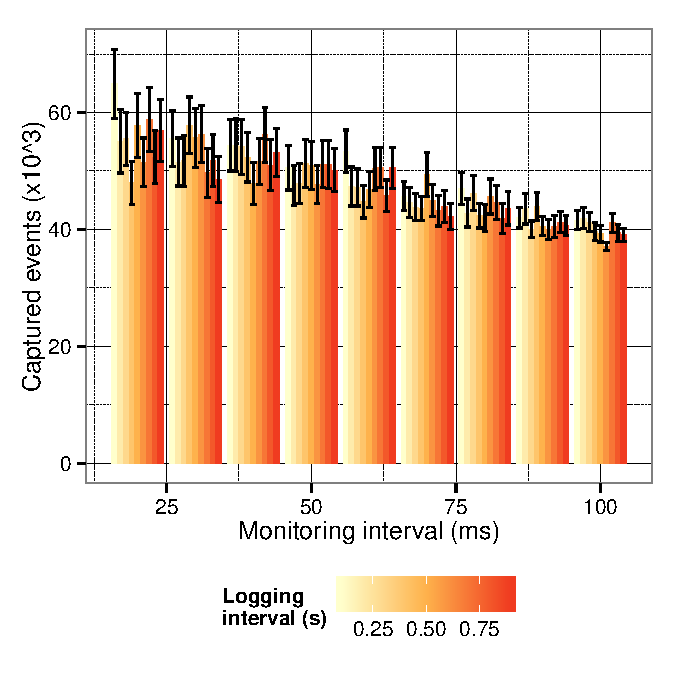
\includegraphics[width=\linewidth]{moca_param_events.pdf}
        \caption{Number of captured events.}
        \label{fig:param_evts}
    \end{subfigure}
    \caption{Influence of the wakeup intervals on \IS, class A.}
    \label{fig:param}
\end{figure}

We can see on the \fig{fig:param_time} that the execution time decreases when we
reduce the monitoring wakeup interval, at \SI{40}{ms}
it seems to reach its worst level, thus we should keep it larger. At \SI{50}{ms}, the
\fig{fig:param_evts} shows that we obtain more than two thirds of the events captured
at smaller intervals, which seems quite reasonable. Finally for this value, a logging
interval of \SI{0.5}{s} seems to provide a good trade-off  between
execution time and precision.
These two values have been chosen as default values in \Moca.


% \newpage

\subsection{Comparison with existing tools}
\label{sec:expe-ovh}

Preliminary experiments showed us that \Mitos capture by
default way less distinct pages than \TABARNAC and \Moca. Thus, we tried to change \Mitos
sampling period in order to make it capture at most pages as possible, 
we call this version \MitosTun. Surprisingly, its behavior regarding this sampling period
is not monotonous, we had to try many different periods to find the proper one.

The default \MemProf distribution did not work with our experimental setup. With the help
of their support team\footnote{see issue at\\\url{https://github.com/Memprof/scripts/issues/1}}, we managed to make it work  disabling the library used to retrieve
data structures names. For the same reason as for \Mitos our study includes
two version of \MemProf: the default version and \MemProfTun for which we have
increased the sampling rate to its maximum.

Finally our evaluation also differentiate \Moca (kernel module only) from
\MocaPin which also retrieve the data structure information using a Pin
instrumentation, we do this differentiation to evaluate the impact of Pin on
\Moca performances.

We compare the different tools on two aspect: trace precision and induced slowdown. The first experiment compares the tools regarding two criteria:  the
percentage of pages and the number of events captured during the analysis.  We use \TABARNAC as a reference to compute the percentage of captured pages,
because, by design, it computes the number of accesses to all the pages used by the studied application. This metric is representative of coverage of a
monitoring tool, its capacity to outline the whole memory area accesses by the application. Then we compare the tools in terms of number of
captured events.  We show the percentage relative to \Moca, as it is the tool that usually provides the more precise traces. We define one event as one
timestamped access found in the trace file outputted by a tool. According to this definition, \TABARNAC does not capture any events as it only keep one
counter per page and per thread without any temporal informations. Thus, \TABARNAC is excluded from this comparison. The number of events is representative
of the precision of a monitoring tool, its capacity to keep track of all the evolutions of the access patterns during the course of the execution. The idea is
that, the more the tool captures events, the less it misses changes in the access patterns.
The second experiment compares the
slowdown factor of the different tools.  All these experiments have been run on each of the \NPB on class A.

\begin{figure}[htb]
    \centering
    \begin{subfigure}{\linewidth}
        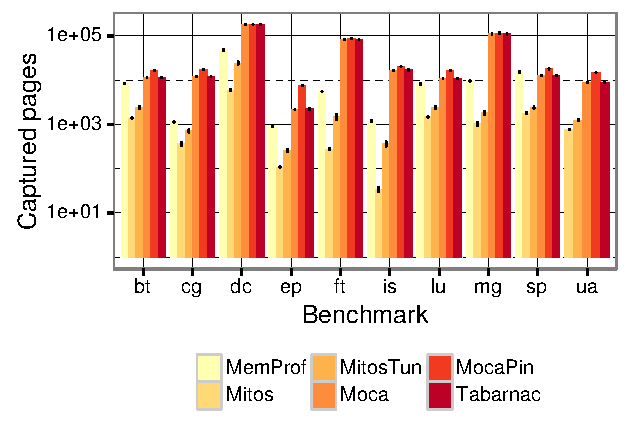
\includegraphics[width=\linewidth]{moca_pages_intel.pdf}
        \caption{Percentage of captured pages.}
        \label{fig:pages}
    \end{subfigure}
    \begin{subfigure}{\linewidth}
        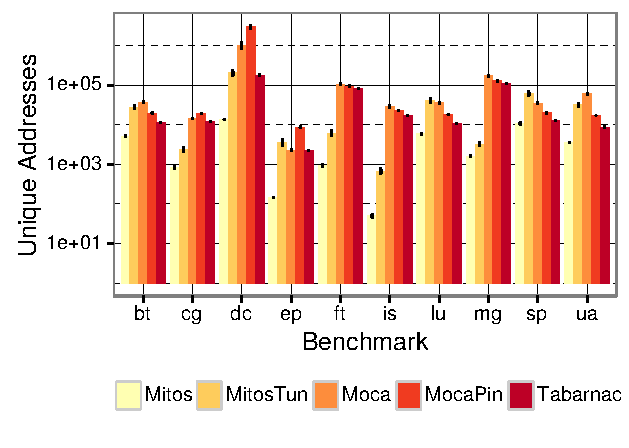
\includegraphics[width=\linewidth]{moca_addr_intel.pdf}
        \caption{Percentages of events captured (compared to \Moca).}
        \label{fig:addr}
    \end{subfigure}
    \caption{Precision of the traces generated by the different tools on the \NPB.}
    \label{fig:pages-addr}
\end{figure}

\fig{fig:pages-addr} presents the results of the precision evaluation of the
different tools. The values used for \Mitos, \MitosTun, \Moca and
\TABARNAC comes from runs on \Edel machines, while \MemProf results comes from
\Stremi.

We can see on \fig{fig:pages} that \Moca captures almost as many pages as \TABARNAC.
Regarding their design they should capture as many pages. Nevertheless, there is a slight
bump in the number of pages used by applications monitored by \TABARNAC due to the Pin instrumentation.
Indeed, its JIT instrumentation recompiles the executable on the fly and changes the memory footprint
(of the stack, mainly). Thus, we can safely ignore these differences and take \Moca as reference.
\DB{Pin indeed modify addresspace, weird stuff: no differences on wheezy}

\Mitos usually collect less than \SI{12.5}{\%} of the pages, adding some fine tunning
can almost double this number but it still misses most of the address space.

Concerning \MemProf, changing the default sampling rate does not seems to
change anything. Both \MemProf and \MemProfTun captures significantly more pages than
\Mitos and \MitosTun. For half of the studied applications it does
not see more than \SI{50}{\%} of the addresses space. Only for, \BT, \LU, \SP and \UA,
which are not the most memory intensive \NPB, 
\MemProf manage capture around \SI{75}{\%} of the accessed pages.
%Finally, for \SP it seems to capture more pages than \TABARNAC and \Moca. As these two reference
%tools uses two different methods to capture all the pages and provide the 
% same number of pages, we can guess that for \SP, which is not a memory
% intensive benchmark, \MemProf capture some system noise in the trace (accesses out
% of the memory space of the process).

From \fig{fig:addr} we can see that, as expected, for almost every benchmarks,
\Moca collects significantly more events than the other tools.  The only
benchmark for which \Moca is not the more precise tool is \EP which is an
Embarrassingly Parallel application with very few memory accesses.
This outlines the fact that \Moca captures events in an uniform way, timed by the monitoring interval.
On the contrary, the other tools might capture more events in a few hotspots presents in the application but miss
sparse accesses during the rest of the execution.
For almost
every other benchmarks both \Mitos (with or without tunning) and \MemProf
hardly reach \SI{10}{\%} of the accesses collected by \Moca, the only exception is
\CG for which \MemProf captures from \SI{25}{\%} to \SI{50}{\%} of the accesses
collected by \Moca.

These results prove that most existing tools can miss a considerable part of
the address-space while \Moca guarantee that it provides a superset of the accessed
pages. Furthermore they show that \Moca is the only existing tool able to provide a
trace precise enough to give an overview of the memory behavior of an application. In
summary, not only our tool provides a complete trace at the granularity of the
page but it is also significantly more precise than the other existing tools.

\begin{figure}[htb]
    \centering
    \begin{subfigure}{\linewidth}
        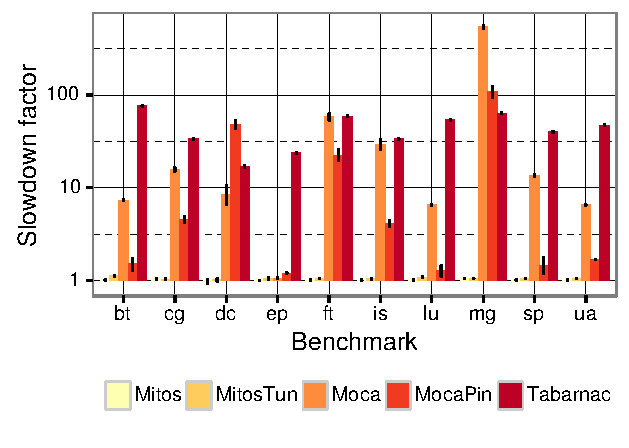
\includegraphics[width=\linewidth]{moca_overhead_intel.pdf}
        \caption{Evaluation on \Edel (Intel)}
        \label{fig:ovh-Intel}
    \end{subfigure}
    \begin{subfigure}{\linewidth}
        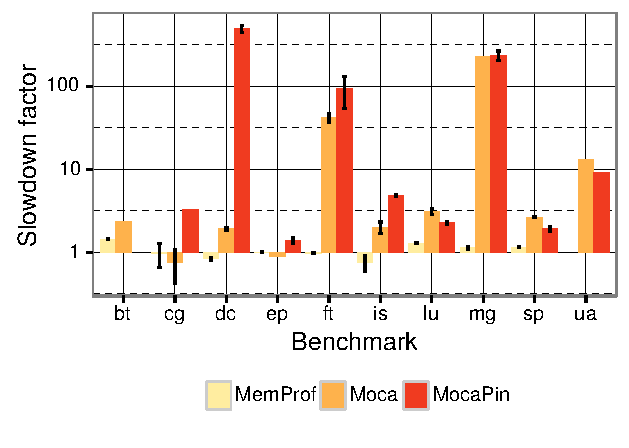
\includegraphics[width=\linewidth]{moca_overhead_amd.pdf}
        \caption{Evaluation on \Stremi (AMD)}
        \label{fig:ovh-AMD}
    \end{subfigure}
    \caption{Slowdown factor of \Moca on the \NPB compared to state of the art tools.
    Y-axis is in log scale.}
    \label{fig:ovh}
\end{figure}

\fig{fig:ovh} shows for each of the \NPB, the slowdown factor when
instrumented by \Moca and the other existing tools on Intel
(\fig{fig:ovh-Intel}) and AMD (\fig{fig:ovh-AMD}) Machines the Y-axis is in
log scale.

From \fig{fig:ovh-Intel}, we can see that \Mitos, \MitosTun overhead is
almost negligible which is not the case for \Moca and \TABARNAC, this
difference is explained by the results of the previous experiment, as these
tools usually collects less than \SI{10}{\%} of the accesses collected by \Moca and
miss a significant part of the address space.

We can classify the benchmarks into three groups:
for \BT, \CG, \DC,  \EP, \LU, \SP and \UA, \Moca is
significantly faster than \TABARNAC. This set of benchmarks is interesting as it is made of varied application profiles.
Indeed, if \EP is mostly doing parallel computation with only a few number of
memory accesses, \CG and \DC are memory intensive and
\BT, \LU as well as \SP are pseudo applications doing a significant usage of memory.
And while \UA is categorised as \emph{unstructured computation,
parallel I/O and data movement} by the \NPB
website\footnote{\url{http://www.nas.nasa.gov/publications/npb.html}}, its
interactions with memory seems noticeable.

The second group only contains memory oriented benchmarks (\FT and
\IS). For this group, \Moca is as good as \TABARNAC or a bit faster, probably
because the balance between computations and memory accesses hides the
overhead of the instrumentation.

For the last benchmark: \MG, \Moca is significantly slower than \TABARNAC. This benchmark
seems to be a pathological case were the execution time with \Moca has a lot a
variability. By looking at our experiment logs, we found that \MG seems to
generate a lot of conflicts on \Moca false page fault hash map. A solution
could be to increase the size of this hash map which is quite difficult as
memory space in the kernel is limited, another easier solution would consist on
working on a smaller version of \MG and see if the analysis is still useful.

\fig{fig:ovh-AMD} shows the results of the evaluation on the AMD machine
(\Stremi). On this machine, \Moca overhead is quite comparable to the results
obtained on \Edel.
For its part \MemProf exhibit a slowdown factor comparable to \Mitos while
providing traces a little more precise. Nevertheless, they are still \emph{incomplete} and
way less precise than \Moca traces. Obviously \MemProfTun have the same
overhead than \MemProf as it capture the same amount of data.

Finally, we can see that as expected, adding one execution under a Pin
instrumentation to retrieve data structures information (\MocaPin) add a small overhead
to \Moca. For several benchmarks this difference is so small that we cannot
differentiate it from \Moca usual overhead.

\subsection{Summary}
\label{sec:expe-cncl}

We have tested \Moca with various applications and using several parameters.
Our experiments, show that \Moca has a good behavior for a wide range of
parameters and helped us defining their default values. Our experiments also
show that, with these parameters, \Moca provides significantly more precise traces
than state of the art tools.
Of course, because of this increased precision, \Moca is slower than two of these tools,
\MemProf and \Mitos.
Nevertheless, the comparison with \TABARNAC outlines the fact that, when a superset of the memory
space is captured, \Moca efficiency is good.
Doing this using \MemProf and \Mitos, and provide the same guarantee, would require to sample all the memory instructions, which is not possible.
At the end of the day, \Moca is the only tool able to provide a
detailed trace with temporal, spacial and sharing information while providing
guarantees on the information lost during the sampling.
